\documentclass[10pt,a4paper]{article}
\usepackage[margin=2.25cm]{geometry}
\usepackage[T1]{fontenc}
\usepackage{lmodern}
\usepackage{amsmath,amssymb,bm}
\usepackage{graphicx,booktabs}
\usepackage{xcolor}
\usepackage[colorlinks=true,allcolors=blue!45!black]{hyperref}
\usepackage{microtype}
\usepackage{placeins}
\graphicspath{{figures/}}
\newcommand{\F}{\bm F}
\newcommand{\E}{\bm E}
\newcommand{\Sg}{\bm S}
\newcommand{\ee}{\bm e}
\newcommand{\ssv}{\bm s}
\newcommand{\dd}{\mathrm d}
\newcommand{\R}{\mathbb R}
\setlength{\emergencystretch}{2em}
\renewcommand{\thesection}{S\arabic{section}}
\renewcommand{\theequation}{S\arabic{equation}}
\renewcommand{\thefigure}{S\arabic{figure}}
\renewcommand{\thetable}{S\arabic{table}}
\title{Supplementary material\\[.4em]\large Physics-augmented neural networks and projection-based reduced-order models for anisotropic hyperelasticity}
\author{}
\date{15 September 2026 --- Working draft}
\begin{document}
\maketitle
\noindent This supplement documents additional SC-RVE constitutive diagnostics---out-of-domain response, sampled finite-strain curvature, and closed-cycle work---together with technical details of the latent-space closure used by the reduced microscopic model. The cycle audit includes both learned constitutive laws and reduced microscopic models.

\section{Out-of-domain constitutive response}
The available SC-RVE fitting data occupy the engineering-strain box
\begin{equation}
 \ee_{\min}=(0,-0.099,-0.168)^T,\qquad
 \ee_{\max}=(0.196,0.016,0.108)^T,
\end{equation}
with $\ee=(E_{11},E_{22},2E_{12})^T$. The independent test set contains 400 states.
An additional 350-state probe extends selected distances from the box center by factors $1.05$, $1.10$, $1.25$, $1.50$, and $2.00$. Five probe labels are nonfinite following failed reference solves and are excluded with the same finite-label mask for all compared models. Their exclusion is reported, not interpreted as proof of a physical instability.
Validation stress selected the compact polyconvex checkpoints before the test and probe responses were evaluated.

Free has aggregate stress errors of $1.2643\%$ on the test set and $5.5024\%$ on the finite probe set. The selected six-feature polyconvex models improve the test fit but do not outperform Free on aggregate probe error. The earlier 32-feature checkpoints extrapolate more accurately than the compact models on this probe, so the $m=6$ selection is restricted to the in-domain coupon deployment. These are not matched-budget architecture comparisons.

\begin{table}[htbp]
 \centering\small
 \caption{SC-RVE: test and probe constitutive errors of the selected six-feature models, in percent.}
 \label{tab:constitutive_probe}
 \begin{tabular}{lrrrrr}
\toprule
Model & $e_S^{\rm test}$ [\%] & $e_W^{\rm test}$ [\%] & $e_S^{\rm probe}$ [\%] & Worst test [\%] & Worst probe [\%] \\
\midrule
ICNN & 0.6214 & 0.1929 & 10.6433 & 4.93 & 114.35 \\
ICKAN & 0.6359 & 0.1900 & 10.0978 & 4.82 & 106.19 \\
\bottomrule
\end{tabular}

\par\smallskip{\footnotesize All values are percentages. The last two columns are maximum per-state stress errors; the first three are aggregate array norms. Test: 400 states; probe: 345 finite reference states out of 350.}

\end{table}

\begin{figure}[htbp]
 \centering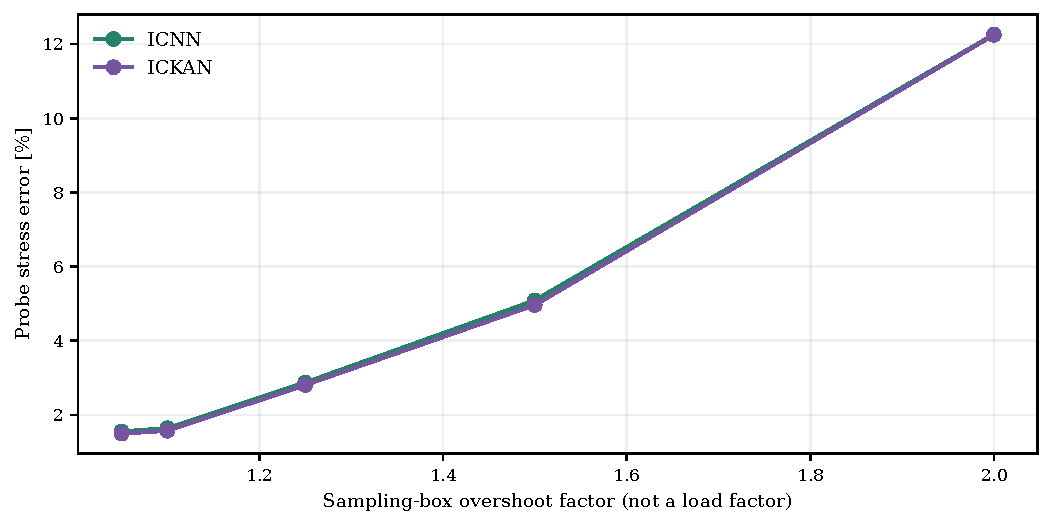
\includegraphics[width=.85\linewidth]{probe_errors.pdf}
 \caption{Stress error on increasingly distant probe rings, using only finite reference labels. Ring factors expand the sampling box; they are not coupon load multipliers. The increase to approximately $19\%$ at factor 2 illustrates a remaining extrapolation limitation despite architectural admissibility.}
 \label{fig:probe}
\end{figure}

\FloatBarrier
\section{Rank-one curvature: samples and an unresolved reference}
For $\bm H=\bm a\otimes\bm b$, the relevant finite-strain curvature is
\begin{equation}
 D^2_{\F}W[\bm H,\bm H]
   =(\delta\ee)^T\bm D\,\delta\ee+\Sg:(\bm H^T\bm H),\quad
 \delta\E=\operatorname{sym}(\F^T\bm H),
 \label{eq:lh}
\end{equation}
where $\delta\ee=(\delta E_{11},\delta E_{22},2\delta E_{12})^T$, $\bm D$ is the engineering-strain stress tangent, and $\Sg$ is the second Piola stress. Here $\bm a,\bm b\in\R^2$ define the rank-one direction and $\operatorname{sym}(\bm A)=(\bm A+\bm A^T)/2$. Omitting the second term tests a different property. In particular, a positive semidefinite tangent with respect to $\ee$ does not generally imply rank-one convexity in compression. For energy-based models, Eq.~\eqref{eq:lh} is evaluated over sampled states and unit directions; negative candidates are checked by second differences of $W(\F\pm h\bm H)$.

\begin{table}[htbp]
 \centering\small
 \caption{Finite rank-one curvature audit. Positive sampled values do not establish a global property.}
 \label{tab:rankone}
 \begin{tabular}{lrrrr}
\toprule
State set & $N$ & Free & ICNN & ICKAN \\
\midrule
Held-out test & 400 & 176.681 & 220.486 & 220.468 \\
Finite-label probe & 345 & 113.034 & 203.280 & 203.538 \\
In-box audit (unlabelled) & 12000 & 163.040 & 213.979 & 211.168 \\
\bottomrule
\end{tabular}

\par\smallskip{\footnotesize Minimum sampled rank-one curvature in MPa. Minima need not occur at the same state or direction. The additional in-box cloud has no independently computed FOM labels; 180 unit directions for $\bm b$ are sampled, with minimization over $\bm a$ via an eigenproblem. None of these finite samples is a global certificate.}

\end{table}

No negative direction is found for Free in the audited test, finite-label probe, and additional in-box sets. An outward search over 1800 strain-space rays finds its first sampled negative value at expansion factor $1.55$, with $J\simeq0.780$ and curvature approximately $-3.43$ MPa. This is a result of that search, not the exact nearest violation. Independent energy finite differences confirm the negative curvature of the learned model.

However, the attempted FOM continuation fails numerically before reaching that candidate. No refined-continuation or global branch-tracking result is available there. Therefore this candidate establishes that the Free network lacks global rank-one convexity, but does not establish disagreement with a converged stable homogenized reference at that state. Solver nonconvergence is not evidence that the physical branch ceases to exist. The stronger claim of an FOM-confirmed false instability is left open. The ICNN and ICKAN have an analytical polyconvexity argument; their sampling audit is a check of implementation, not its replacement.


\FloatBarrier
\section{Closed-cycle work of the effective stress}
\label{sec:cycle}
For a hyperelastic law, returning to the same deformation on the same reversible equilibrium branch returns the stored energy to its initial value. The net stress work must therefore vanish:
\begin{equation}
 \mathcal W_{\rm cyc}=\oint\ssv\cdot\dd\ee=0,
 \qquad
 \ee=(E_{11},E_{22},2E_{12})^T,\quad
 \ssv=(S_{11},S_{22},S_{12})^T.
\end{equation}
Here $\ee$ and $\ssv$ are work-conjugate strain and stress vectors. A nonzero result beyond numerical error rules out an exact potential for that stress map; a zero result on one cycle cannot establish one. The test does not assess polyconvexity.

We use a rectangle of half-width $0.001$ in $(E_{11},E_{22})$, with fixed shear and center
\[
 \ee_c=(0.0051260033,-0.0945507613,-0.1283720602)^T.
\]
It lies inside the SC-RVE fitting box. The center was selected after observing Regression tangent asymmetry; the same cycle was subsequently applied to the frozen reduced models.

\begin{table}[htbp]
 \centering\small
 \caption{Net work around the counterclockwise SC-RVE cycle, in J m$^{-3}$.}
 \label{tab:cycle}
 \begin{tabular}{lr}
 \toprule
 Model & $\mathcal W_{\rm cyc}$\\
 \midrule
 FOM & $-6.98\times10^{-10}$\\
 Regression & $-213.922$\\
 Free & $2.34\times10^{-10}$\\
 ICNN & $4.02\times10^{-10}$\\
 ICKAN & $1.09\times10^{-5}$\\
 HPROM & $-1.234$\\
 HPROM--ANN & $247.774$\\
 D--HPROM--ANN & $54.082$\\
 \bottomrule
 \end{tabular}
 \par\smallskip{\footnotesize 128 Gauss points per edge; FOM uses 8. The ICKAN residual decreases with quadrature refinement through its spline knots.}
\end{table}

Free, ICNN, and ICKAN obtain stress by differentiating an energy; their residuals are consistent with numerical integration and roundoff. Regression and the deployed HPROM outputs retain nonzero work under quadrature refinement. Reversing the cycle reverses its sign, and tighter equilibrium tolerances leave the intrusive residuals essentially unchanged.

The HPROMs fit equilibrium and stress cubatures separately, so their effective stresses are not guaranteed to derive from one energy. This diagnostic concerns those implementations. Among them, the largest ratio of absolute net work to accumulated absolute work along this cycle is $0.0205\%$. Its effect on coupon accuracy has not been demonstrated. The selected cycle establishes neither a general ranking of the models nor the frequency of such defects across the strain domain.

\end{document}
